\section{What is Science?}

\begin{frame}
  \begin{center}
    Part I: What is Science?
  \end{center}
\end{frame}

\subsection{Definitions}
\begin{frame}{What is Science?}
  At the end of your 2-year course, you will receive a diploma that says:
  \begin{center}
    Master in Computer \structure{Science}
  \end{center}
  What does that word mean?
  \bigskip

  \begin{block}<2>{Some answers from students in past years}
    \begin{itemize}
      \item Science is a method to learn about the world;
      \item Science is a method to reach the truth;
      \item Science is useful when it contributes to society;
      \item Science is how we develop new technologies;
    \end{itemize}
  \end{block}\bigskip

  Give me {\bf your} answer on manaba!
\end{frame}

\begin{frame}{What is Science}{(Not) answering the question}
  \begin{itemize}
    \item All of the answers in the last slide are correct;
    \item "Science" may mean different things to people, depending on their background;
    \item But even the different answers have some common characteristics:
    \begin{itemize}
      \item The discovery of new knowledge;
      \item Understanding the natural world;
      \item Focus on correctness and methodology;
    \end{itemize}
    \item There are also some characteristics that are not often discussed
    \begin{itemize}
      \item Science as a {\bf community}
      \item Science as a {\bf continuous process}
      \item The relationship between {\bf science and society}
    \end{itemize}
  \end{itemize}
\end{frame}

\begin{frame}{What is Science}{I know it when I see it}
  One way that I like to use to understand science, is to look at people who are doing it, and think about what they do.\bigskip

  I think it is important for us to inspire ourselves on the work of other scientists. It is good to have heroes!\bigskip

  So let's talk about \structure{Marie Curie}
\end{frame}

\subsection{Marie Curie}
\begin{frame}{Marie Curie}{Fact Sheet}
  \begin{columns}
    \column{.3\textwidth}
  \includegraphics[width=1\textwidth]{../img/irasutoya_curie}
  \ppagenote{Marie Curie sketch from \url{https://www.irasutoya.com}}\\
    \column{.7\textwidth}

    \begin{itemize}
      \item From Poland, born in 1867, died in 1934.
      \medskip

      \item Physicist and Chemist
      \medskip

      \item Pioneer of radioactivity
      \medskip

      \item First woman to win the Nobel Prize
      \medskip

      \item Only woman to win the Nobel Prize \alert{Twice}
      \medskip

      \item Only person to win the Nobel Prize\\
      \alert{In two different fields}\\
      (Physics and Chemistry)
    \end{itemize}
  \end{columns}
\end{frame}

\begin{frame}{Marie Curie}{Humble Beginnings}
  \begin{columns}
    \column{0.3\textwidth}
    \includegraphics[width=1\textwidth]{../img/marie_curie_sister}\ppagenote{Curie sisters image from Wikipedia (public domain)}\\
    Marie Curie and her sister
    \column{0.7\textwidth}
  \begin{itemize}
    \item Born in Poland
    \medskip

    \item Could not enroll at the local university;\\
      (only accepted men at the time)\medskip

    \item Got educated at the clandestine "Flying University"
    \medskip

    \item Worked as a tutor and home teacher to sustain herself;
  \end{itemize}
\end{columns}
\end{frame}

\begin{frame}{Marie Curie}{Moving to Paris}
  \hfill\includegraphics[width=.3\textwidth]{../img/marie_pierre_curie}\ppagenote{Marie and Pierre Curie image from Wikipedia (Public Domain)}
  \begin{itemize}
    \item Moved to Paris and earned a Physics Degree;

    \item As a researcher, worked in a small shed;
    \item Had difficulty finding research money (funding);
  \end{itemize}
\end{frame}

\begin{frame}{Marie Curie}{Research in Radiology}
  \begin{itemize}
    \item In Marie Curie's time, there was a lot of interest in radioactive materials;
    \begin{itemize}
      \item Why did some materials emit radiation?
      \item What was radiation?
      \item What could we use it for?
    \end{itemize}\bigskip

    \item One of her significant discoveries was that the quantity of radiation depends only on the amount of material;
    \begin{itemize}
      \item This meant that radiation was an \structure{innate property} of radioactive material, not something that was acquired.
    \end{itemize}\bigskip

    \item Marie Curie did not patent the techniques she discovered to study radioactive materials, so that other scientists could also improve their work, and science could progress even faster.
  \end{itemize}
\end{frame}

\begin{frame}{Marie Curie}{Applications of her research}
  \begin{itemize}
    \item Observed that tumour cells died more quickly to radiation than healthy cells;
    \medskip

    \item Developed mobile X-Ray units to be used for surgery during World War I ("little curies")
    \medskip

    \item Developed "Radium Needles" for sterilizing tissue;
  \end{itemize}
  \hfill\includegraphics[width=0.3\textwidth]{../img/irasutoya_ambulance.png}
  \ppagenote{Ambulance from \url{https://www.irasutoya.com}}
\end{frame}

\begin{frame}{Marie Curie}{Legacy}
  Unfortunately, Marie Curie died early from radiation damage, like many scientists of the time. Her research notebooks are still radioactive, and must be held in special containers!\vfill

  What can you learn from the history of Marie Curie?\bigskip

  What are the scientists that you know? or that inspire you. What can you learn from their history?
\end{frame}

\subsection{Scientific Discoveries}
\begin{frame}{What is Science?}{Scientific Discoveries}
  Science comes in many different forms.\vfill

  Let's discuss two interesting and very different scientific discoveries:
  \begin{itemize}
    \item The cosmic background radiation;
    \item Citrus fruits and scurvy;
  \end{itemize}
\end{frame}

\begin{frame}{The Origins of the Universe}
  \begin{itemize}
    \item Physics is a discipline interested in explaining how the universe works. One question of particular interest to physicists is \structure{how the universe began}.\bigskip

    \item One of the most well supported theories for the beginning of the universe is the "inflation theory". According to inflation, the universe started as very dense plasma, and then there was a period of very quick expansion and cooling.\bigskip

    \item Why is the "inflation theory" considered to be well supported? How can we know what happened in the beginning of the universe?
  \end{itemize}
\end{frame}

\begin{frame}{The Origins of the Universe}{What evidence supports "inflation"?}

  \begin{columns}

    \column{0.6\textwidth}
    \begin{itemize}
      \item "Inflation Theory" predicted was that for a very short moment,  the universe had expanded enough to be transparent, but was still hot enough to glow.\medskip

      \item The theory allowed a calculation of the duration and intensity of this glow, and that it would be observed from all directions at once.\medskip

      \item Many years later, astronomical radiations actually found evidence for this glow, by accident, which confirmed the theory.\medskip
    \end{itemize}

    \column{0.4\textwidth}
    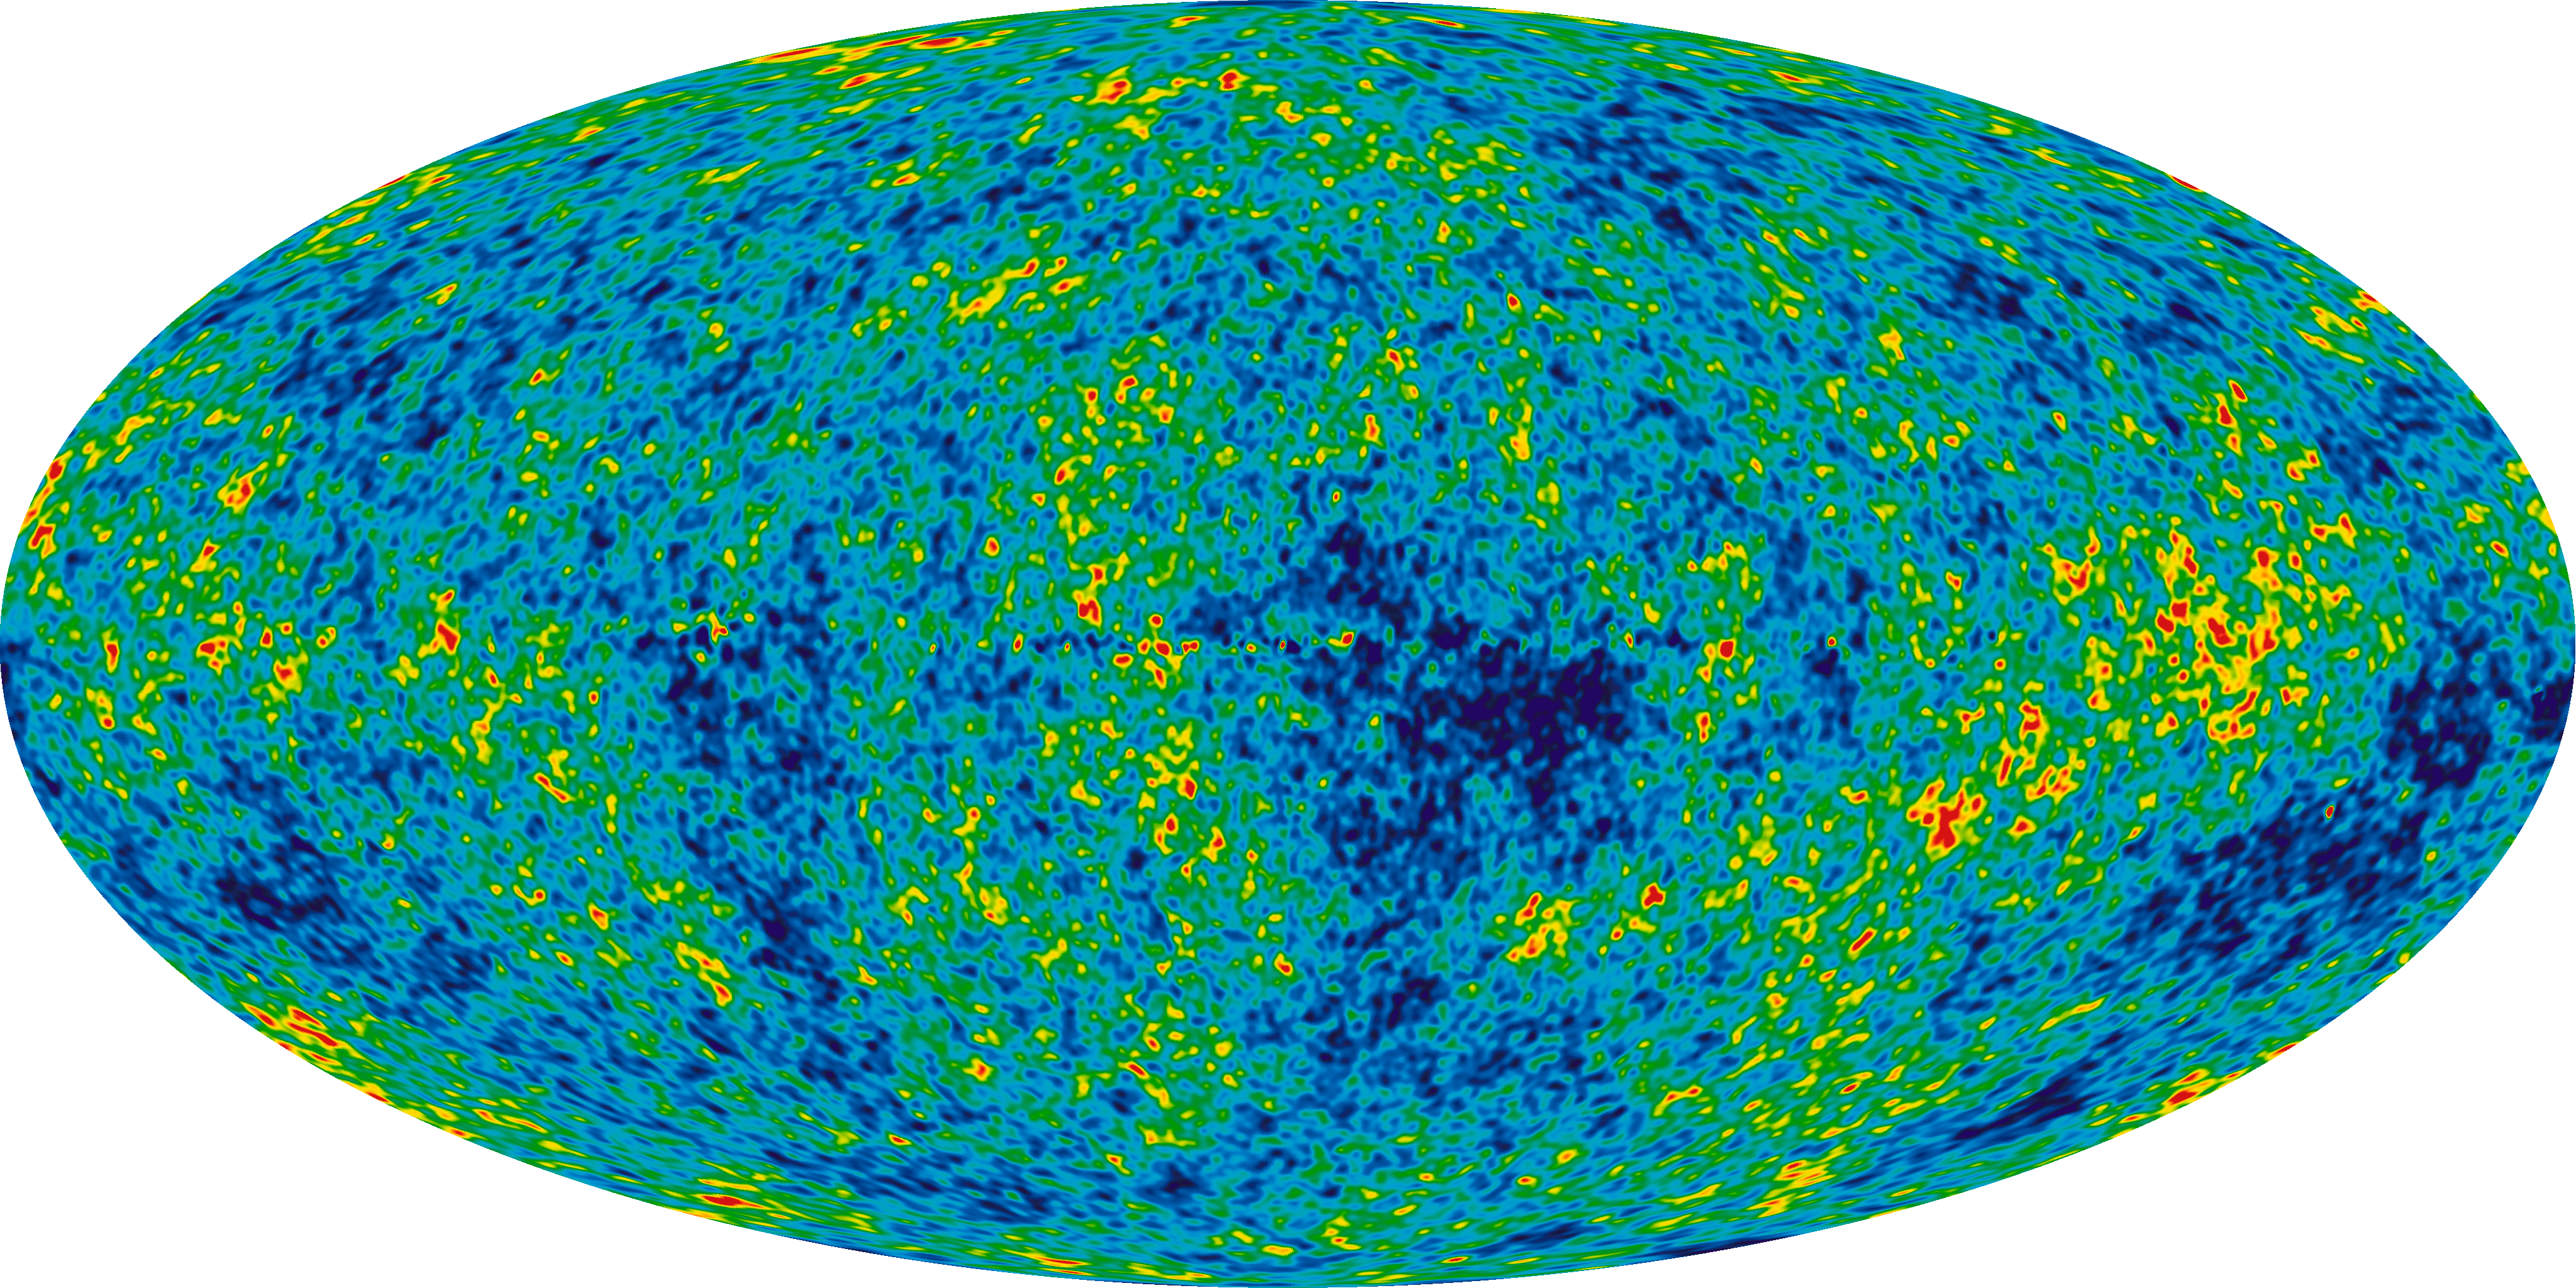
\includegraphics[width=1\textwidth]{../img/nasa_cmb}
    \includegraphics[width=1\textwidth]{../img/nasa_cmb_data}\\
    \ppagenote{CMB images from NASA (public domain)}

  \end{columns}
\end{frame}

\begin{frame}{Citrus fruits and scurvy}
  In the 18th century, the British Empire had a very large fleet of ships plundering the entire world.\bigskip

  Maintaining the health of sailors during these long trips was an important issue.\bigskip

  \structure{James Lind}, a scottish doctor, pioneered several ideas to improve naval hygiene. Among those, he conducted a trial to discover how to prevent {\bf scurvy} among sailors.
\end{frame}

\begin{frame}{Examples of Scientific Discoveries}{Citrus fruits prevents scurvy}
  \begin{center}
    \includegraphics[width=1\textwidth]{../img/wikipedia_scurvy}
    \ppagenote{James Lind image from Wikipedia, Public Domain}
  \end{center}
\end{frame}

% TODO
\subsection{The Scientific Method}
\begin{frame}{The Scientific Method}{}
  \begin{columns}
    \column{0.5\textwidth}
    \begin{itemize}
      \item The examples we saw demonstrate the familiar idea of the scientific method;
      \bigskip

      \item Hypothesis, {\bf Experiment}, Analysis;
      \bigskip

      \item But is this really all that there is to the scientific method?
    \end{itemize}
    \column{0.5\textwidth}
      \includegraphics[width=1\textwidth]{../img/scientific_method_simple}
  \end{columns}
\end{frame}

%TODO
\begin{frame}{The Scientific Method}{Science as an interactive process}
  The scientific process can be more complex than a simple recipe.
  \begin{center}
    \includegraphics[width=0.7\textwidth]{../img/interactive_science}\ppagenote{Image from "understanding science, University of berkerley"}
  \end{center}
\end{frame}

% TODO
% What about computer science?
%% Can we use computers as a tool to understand the world better?
%% Can we improve the world using computers?
%% Can we understand computer systems better to improve their capacity?
%% Can we change how we understand the world, but using computer systems?
